\documentclass{book}

\usepackage{graphicx,amscd,amsmath,amssymb,verbatim}
%\usepackage[dvips]{hyperref}	% for hyperlinks
\usepackage{url}
\usepackage{epstopdf} % so can use EPS or PDF figures
\usepackage{appendix}	% for finer control of the appendix

\DeclareMathSymbol{\Gamma}{\mathalpha}{letters}{"00}	% Greek capital letters in italics
\DeclareMathSymbol{\Delta}{\mathalpha}{letters}{"01}
\DeclareMathSymbol{\Theta}{\mathalpha}{letters}{"02}
\DeclareMathSymbol{\Lambda}{\mathalpha}{letters}{"03}
\DeclareMathSymbol{\Xi}{\mathalpha}{letters}{"04}
\DeclareMathSymbol{\Pi}{\mathalpha}{letters}{"05}
\DeclareMathSymbol{\Sigma}{\mathalpha}{letters}{"06}
\DeclareMathSymbol{\Upsilon}{\mathalpha}{letters}{"07}
\DeclareMathSymbol{\Phi}{\mathalpha}{letters}{"08}
\DeclareMathSymbol{\Psi}{\mathalpha}{letters}{"09}
\DeclareMathSymbol{\Omega}{\mathalpha}{letters}{"0A}

%%%%%%%%%%%%%%%%%%%%%%%%%%%%%%%%%%%%%%%%
%%%%%%%%%%%%%%%%%%%%%%%%%%%%%%%%%%%%%%%%
\begin{document}

\frontmatter

\begin{titlepage}
	\begin{center}

		\huge{Avalanches, Brains and Stocks: Simulating Self-Oraganised Criticality}

		\vspace{2.5cm}

		\LARGE{Avi Vajpeyi}\\ 
		\LARGE{Physics and Computer Science Departments}\\
		\LARGE{The College of Wooster}\\
		
		\vspace{0.5cm}
		
		\large A dissertation submitted in partial fulfillment 
		of the requirements of  Senior Independent Study in Physics at The College of Wooster\\
		
		\vspace{2.5cm}
		
		\begin{table}[h!]
			\begin{center}
				\begin{tabular}{c}
				
					\large{\emph{Physics Adviser}}\\
					\large{Dr. John F. Lindner}\\
					\vspace{0.5cm}\\
					\hline
					
					\vspace{1.0cm}\\
					\large{\emph{Computer Science}}\\
					\large{Dr. Denise Byrens}\\
					\vspace{0.5cm}\\
					\hline
					
				\end{tabular}
			\end{center}
		\end{table}
		
		\vspace{2.5cm}

		\large{\today}

	\end{center}
\end{titlepage}

%%%%%%%%%%%%%%%%%%%%%%%%%%%%%%%%%%%%%%%%
\chapter*{Abstract}\addcontentsline{toc}{chapter}{Abstract}
\indent Experiments with a granular bead pile have shown that the pile can model critical systems such as avalanches. In the experiments, a bead is dropped on the apex of the pile of beads. Eventually, one such bead causes several beads of the conical bead pile to avalanche. The experiments have studied the distribution of avalanches and how the distribution is affected by altering the bead type, bead cohesion, and bead drop height. In this study we present a computational simulation of the experiment.\\
 \indent The simulation models each bead as independent particles with their own positions and velocities. The internal and external forces on each particle are accumulated to provide the new particle positions using Newton's second law of motion. As each particle is independent, we can use parallelism to thread various processes of the particles to the graphical processing unit. This allows the simulation run in real-time while still having $60$k particles on the pile.\\
\indent With this simulation we can learn new information from the system that may have been challenging to study with the actual experiment. For example, we can vary the shapes and numbers of the beads. With the simulation it is also possible to record the velocity of each particle both on the surface and inside the pile. 

%%%%%%%%%%%%%%%%%%%%%%%%%%%%%%%%%%%%%%%%
%\chapter*{Acknowledgments}\addcontentsline{toc}{chapter}{Acknowledgments}
%I would like to thank Dr. Lindner and Dr.

%%%%%%%%%%%%%%%%%%%%%%%%%%%%%%%%%%%%%%%%
%%%%%%%%%%%%%%%%%%%%%%%%%%%%%%%%%%%%%%%%
\tableofcontents
\setcounter{tocdepth}{2}
\listoftables
\listoffigures

%%%%%%%%%%%%%%%%%%%%%%%%%%%%%%%%%%%%%%%%
%%%%%%%%%%%%%%%%%%%%%%%%%%%%%%%%%%%%%%%%
%%%%%%%%%%%%%%%%%%%%%%%%%%%%%%%%%%%%%%%%
\mainmatter

%%%%%%%%%%%%%%%%%%%%%%%%%%%%%%%%%%%%%%%%
%%%%%%%%%%%%%%%%%%%%%%%%%%%%%%%%%%%%%%%%
\chapter{Introduction}\label{introduction}
%discussion of everything in shallow... 
\section{Per Bak and Sand in Brains}
\subsection{Background}
In 1999 a Danish scientist by the name Per Bak explained the disordered electrical neural activity of a brain in an audacious way that left many neurologists puzzled \cite{MindSandWeb}.  He suggested that the brain's neural activity worked in a similar way as a sand pile upon which avalanches of varying sizes occur to maintain stability -- instabilities paradoxically helping provide the system with stability \cite{MindSandWeb}. As more sand is added to the pile, more avalanches occur along the surface of the conical shape. Some of the avalanches are large and cause the sand to slip off the pile. Smaller avalanches lead to the sand grains sliding down a short distance before coming to a stop, as seen in Figure~\ref{fig:sandPileModel}. 

	\begin{figure*}[h]
	\centering
	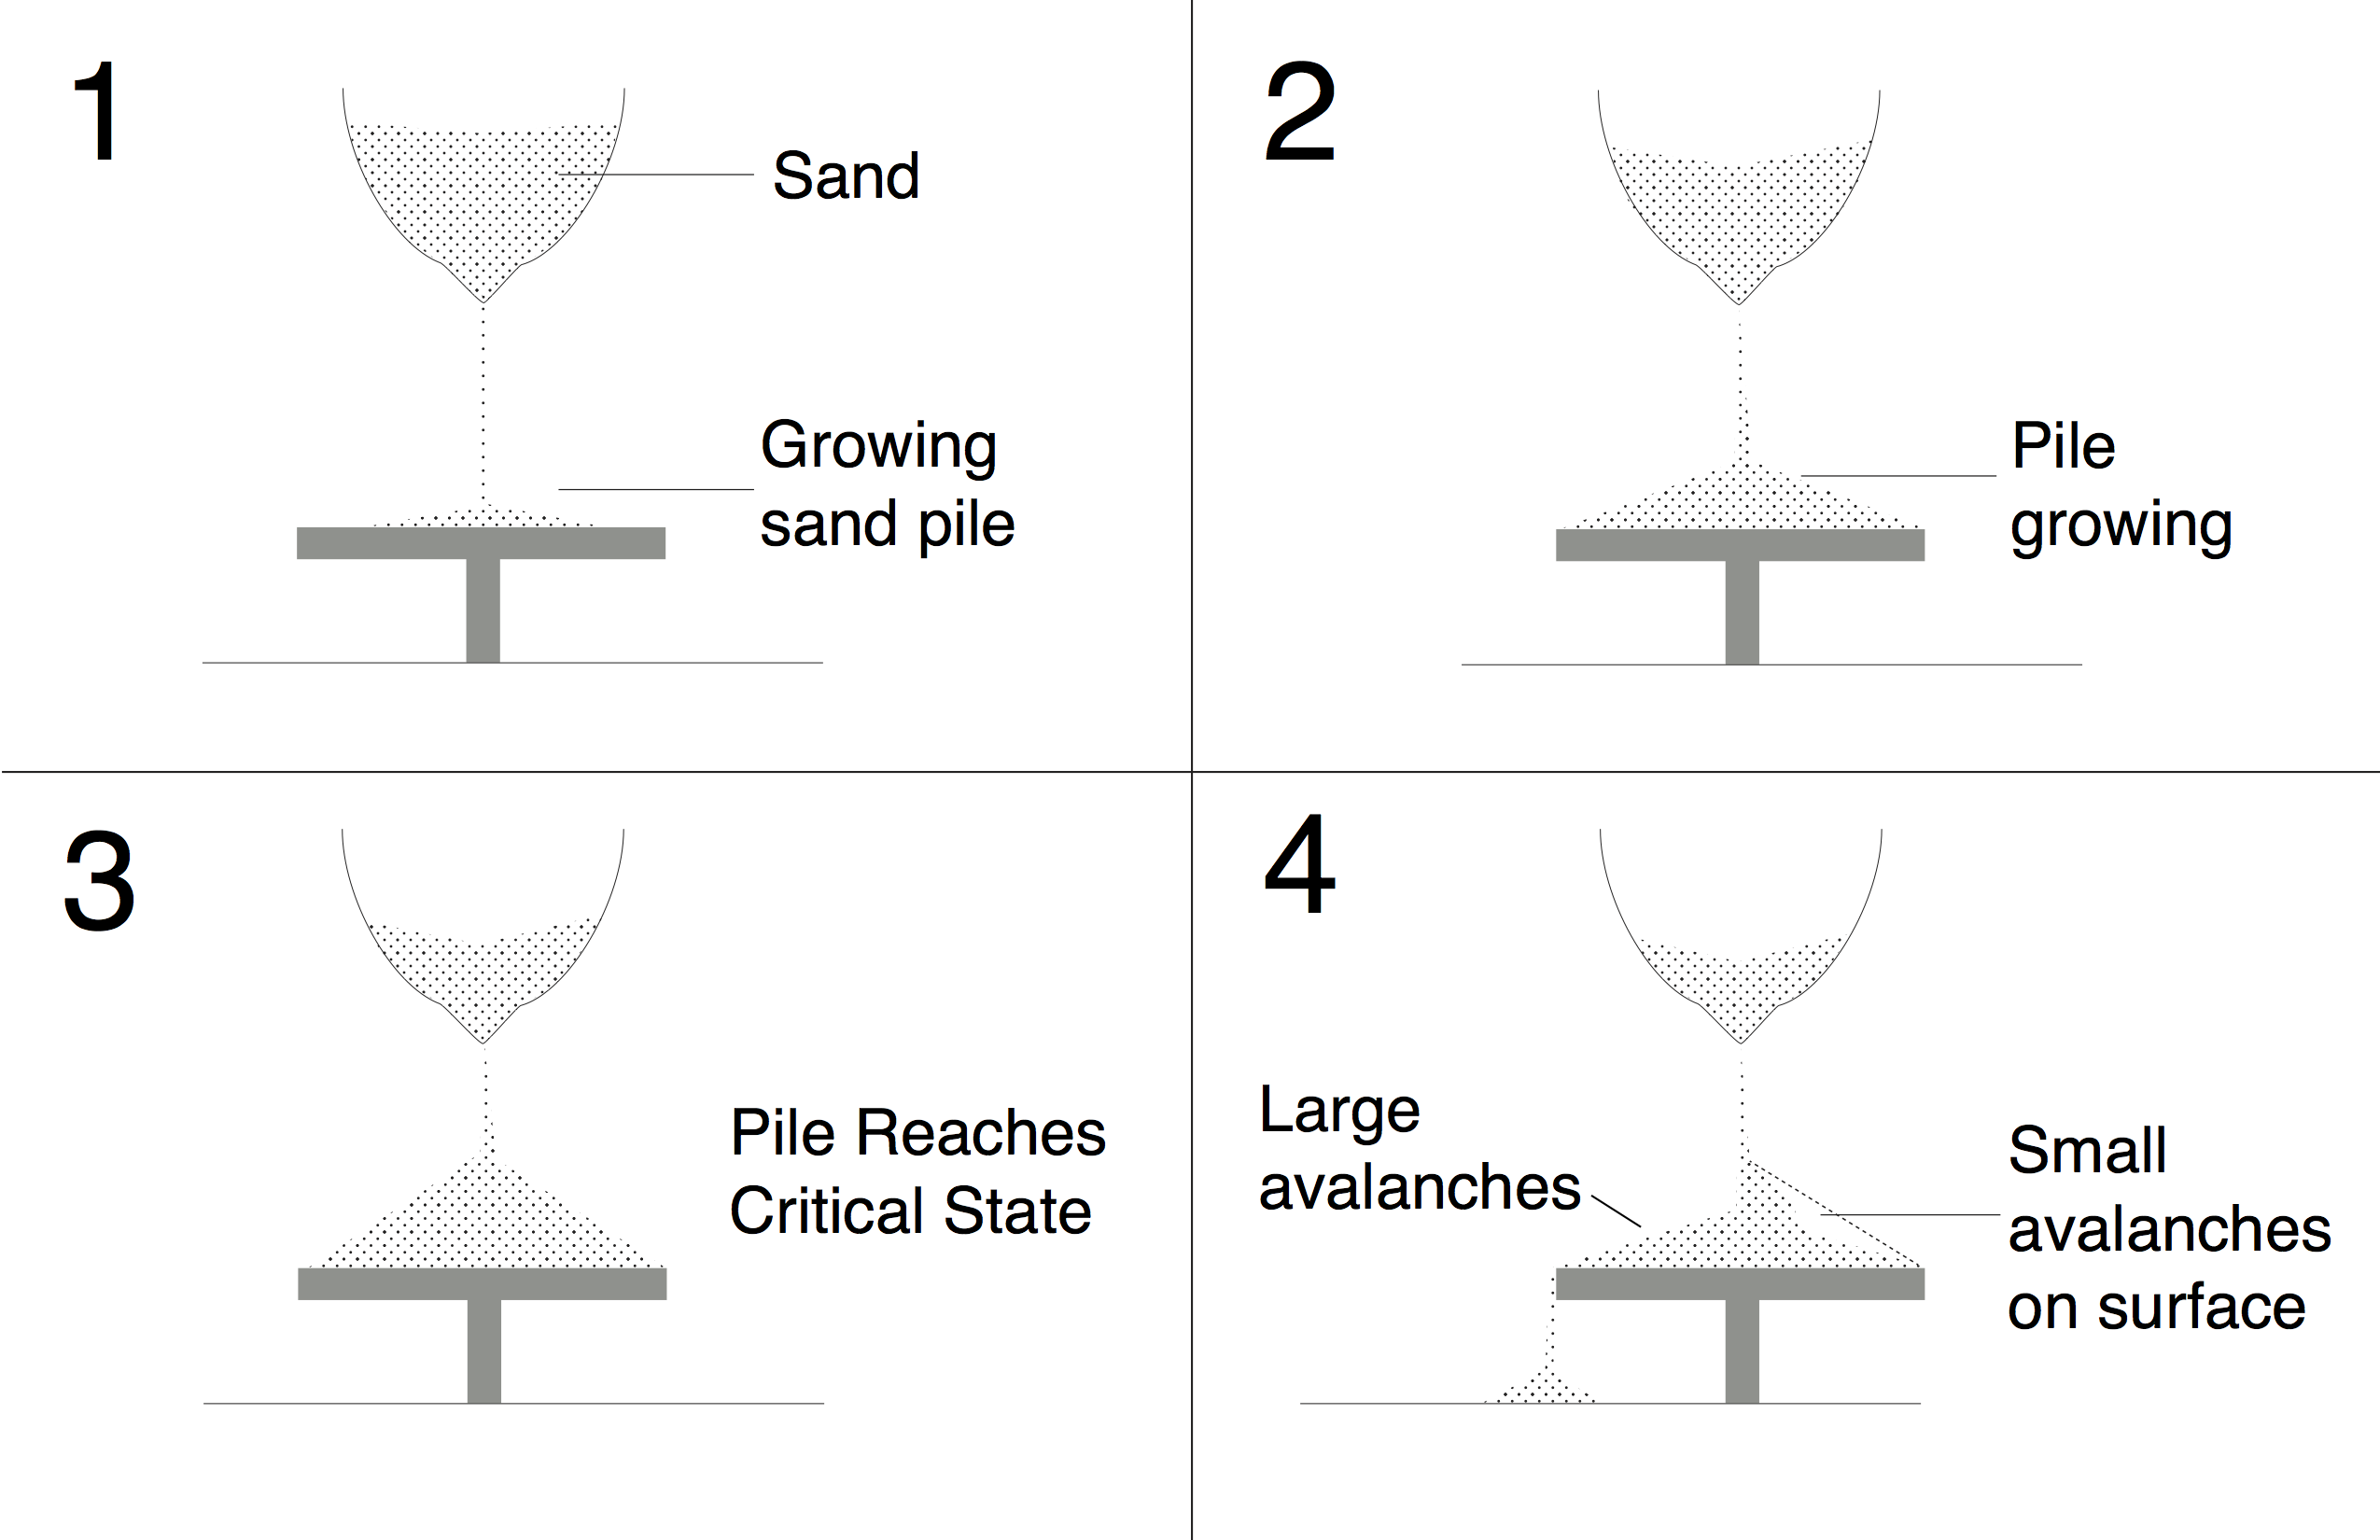
\includegraphics[width=0.8\textwidth]{Figures/Intro/SandPileFigs/sand_pile_model.png}
	\caption[Per Bak's Theoretical Sand Pile Model]{
		\textit{Per Bak's Theoretical Sand Pile Model:} Sand is dropped regularly on a flat surface. The sand piles up in a conical shape and eventually reaches a critical point. At the critical point, the addition of even a single grain can lead to an avalanche. This image was modified from one seen in \cite{IMGSandPile}.}
	\label{fig:sandPileModel}
\end{figure*}

Even with these unpredictable avalanches, the conical shape of the pile is maintained. Per Bak pointed out that although the individual avalanches were unpredictable in timing and size, the \textit{distribution} of the timings and sizes of several avalanches \textit{demonstrate a regularity} \cite{OGperBak1987}. He coined the term ``self-organised criticality'' (SOC) as this phenomena of finding order in systems which appeared to be unpredictable.  He explained to the neurologists that perhaps brains, like sand piles, behave as self-organised critical systems \cite{MindSandWeb}. This is because the disordered electrical activity of neurons which permits us to think spontaneously arises from some ordered complexity \cite{MindSandWeb}. 


\subsection{The Origins of SOC: Critical Points}
In the 1980s, Bak began studying phase transitions in the hopes of better understanding how it is possible to find order in nature which is made up of disordered particles \cite{MindSandWeb}. Phase transitions, the process by which matter transforms from one phase into another, can involve a sudden change (like the magnetization of ferro-magnets), or it can involve a gradual change (like ice transitioning to water) \cite{PhaseTransitionInfo}. In any transition, there is a precise moment called the tipping or critical point at which the matter is halfway between each phase (see Figure~\ref{fig:critPoint} to look at a phase diagram of carbon dioxide with it's critical point marked).

\begin{figure*}[h]
	\centering
	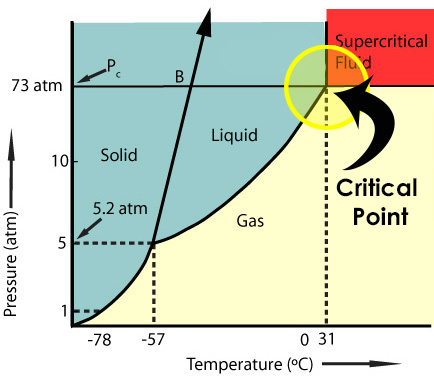
\includegraphics[width=0.5\textwidth]{Figures/Intro/SandPileFigs/critical_co2}
	\caption[CO$^2$ phase diagram]{
\textit{CO$^2$ phase diagram:} the critical point for CO$^2$ to transition from liquid/gas/super-fluid is marked on the plot. This image was taken from \cite{IMGCriticalPoint}. 
}
	\label{fig:critPoint}
\end{figure*}


 In the case for most phase transitions, there are certain criteria that need to be met before matter can transition to another phase. For example - the local temperate and pressure must be within a specific range for ice to transition into water. Studying these transitions, which can be reached only with the tuning of parameters, led Bak to study transitions that require no fine tuning of parameters \cite{MindSandWeb}. He observed that in such transitioning systems, interactions of local elements of the system could spontaneously bring the system to a critical point -- a self-oraganised critical point. He demonstrated the existence of SOC behavior with a simulation of a sandpile which he and his colleagues implemented using a cellular automata \cite{OGperBak1987}. 
\subsection{The Sandpile Cellular Automata}
In the simulation presented in \cite{OGperBak1987}, as sand is added to the pile, the local slopes on the pile increase (where the slopes are the cellular variables that evolve the cellular automata). If the slope is steep enough to overcome the the static friction holding the grains to the sides of the conical pile, grains slide down to neighboring positions. If the slope at the neighboring positions are also greater than the force required to hold the grain,  the grain can continue to slide down the side of the pile.  Eventually, the avalanche of sliding grains comes to a halt when the grains settle in positions where they can remain. Figure~\ref{fig:perBak_cellular} shows a state of the sandpile produced from the group's cellular automata while Figure~\ref{fig:ConceptualSandpileModel}is the conceptual model of the sandpile that this simulation is made from. 
\begin{figure*}[h]
	\centering
	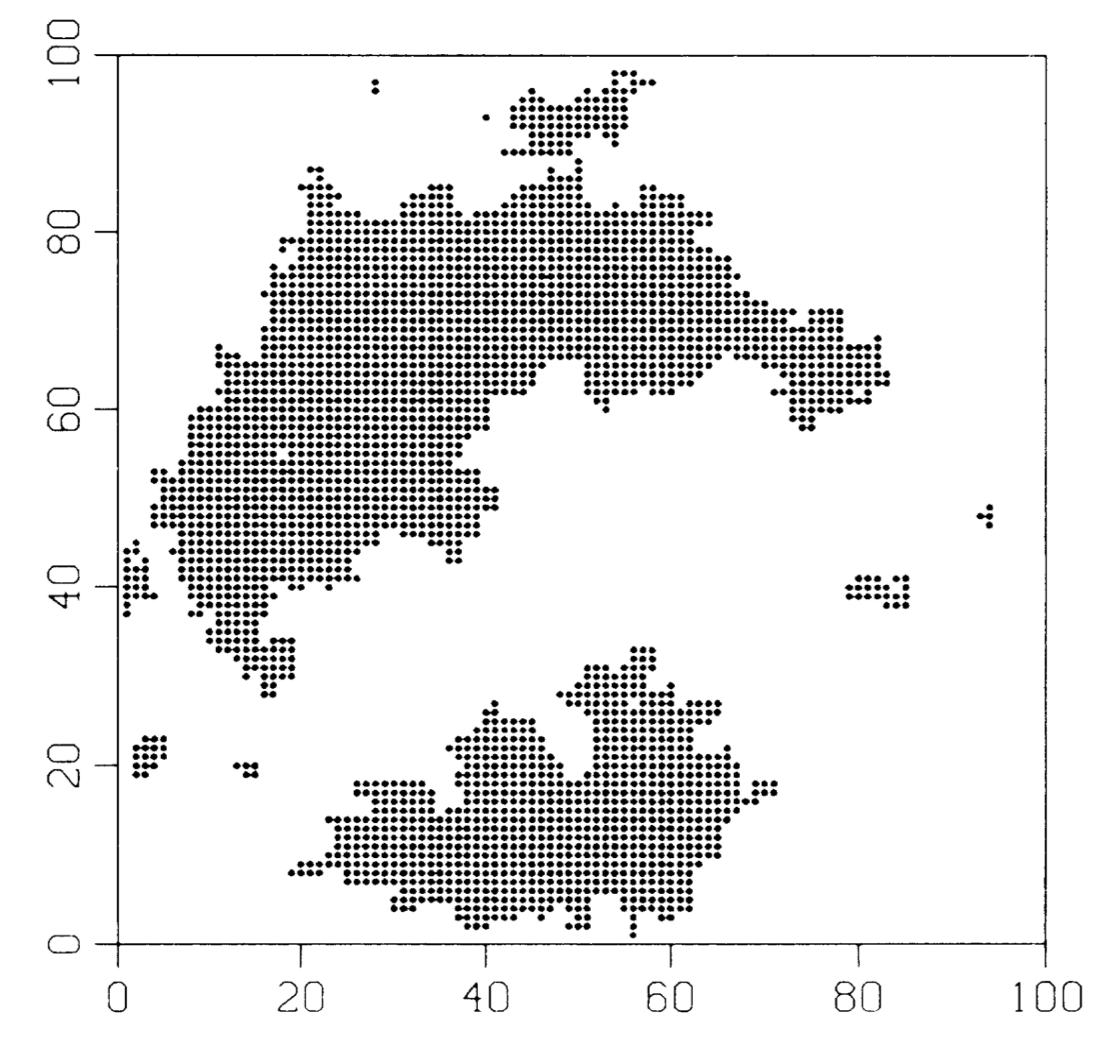
\includegraphics[width=0.4\textwidth]{Figures/Intro/SandPileFigs/perBak_cellular}
	\caption[Snapshot of the sandpile cellular automata]{
		\textit{Snapshot of the sandpile cellular automata:} this snapshot was generated from a cellular automata of dimensions 100 by 100. The dark regions represent clusters that have been affected by the dropping of a single grain of sand at a point.  This image was taken from \cite{OGperBak1987}.}
	\label{fig:perBak_cellular}
\end{figure*}
\begin{figure*}[h]
	\centering
	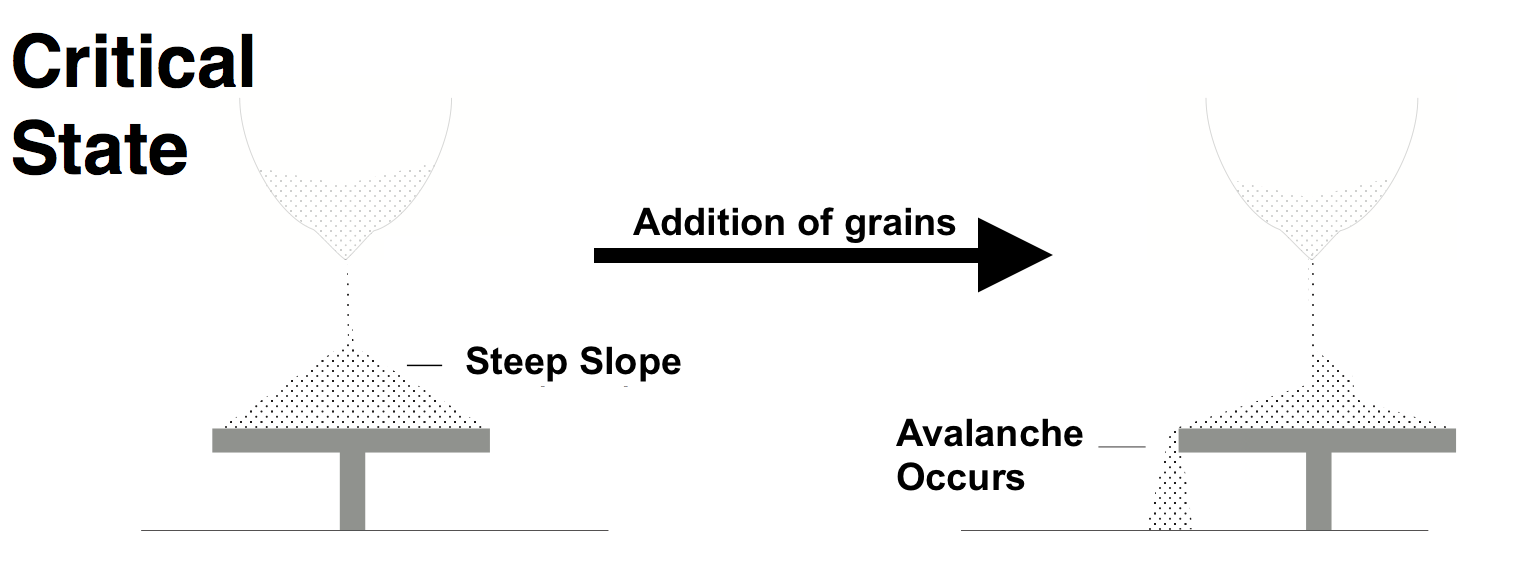
\includegraphics[width=0.8\textwidth]{Figures/Intro/SandPileFigs/theoreticalModel}
	\caption[Conceptual model of Bak's Sandpile Simulation]{
		\textit{Conceptual model of Bak's Sandpile Simulation:} When the pile is critical, then the addition of even a single grain can lead it to avalanche. This image was created using a similar style as in \cite{IMGSandPile}.}
	\label{fig:perBak_cellular}
\end{figure*}
Per Bak and his colleagues published the paper on the sand pile simulation and SOC in 1987. Soon afterward, Bak even published a book titled \textit{`How Nature Works'} \cite{howNatureWorks}. In the book, Bak extends the concept of SOC and demonstrates its presence in other complex systems ranging from financial markets,  forest fires, evolution, earthquakes, galaxy distributions and even the brain \cite{howNatureWorks} (further work on how these systems demonstrate SOC behavious can be found here in order of the different systems mentioned \cite{stockMarketProof, ForestFireProof,evolutionProof,EarthquakesProof,galaxyFormationProof,BrainProof}). According to Bak, these systems lie on the fence separating order from disorder. Bak was able to study these complex systems only with simulations and so other scientists were still skeptical of his hypotheses about SOC \cite{MindSandWeb}. Some considered his work to be too simplistic and unable to capture the intricacies of realistic systems \cite{MindSandWeb}. 
\subsection{Experimental Verification}
A little afterwards, in 1992, the physics department of the University of Oslo was able to experimentally test Bak's sand pile model \cite{riceExpt}. In their experiment, they confined grains of rice between two glass plates, as show in Figure~\ref{fig:riceModel}. They added grains till the pile reached a `quasi-stationary' state \cite{riceExpt}. At this stage, they began recording a video of the pile and then continued the grain dropping. When there was an avalanche, they used the video to compare images of the pile before and after the avalanche to calculate the size of the avalanche. 
\begin{figure*}[h]
	\centering
	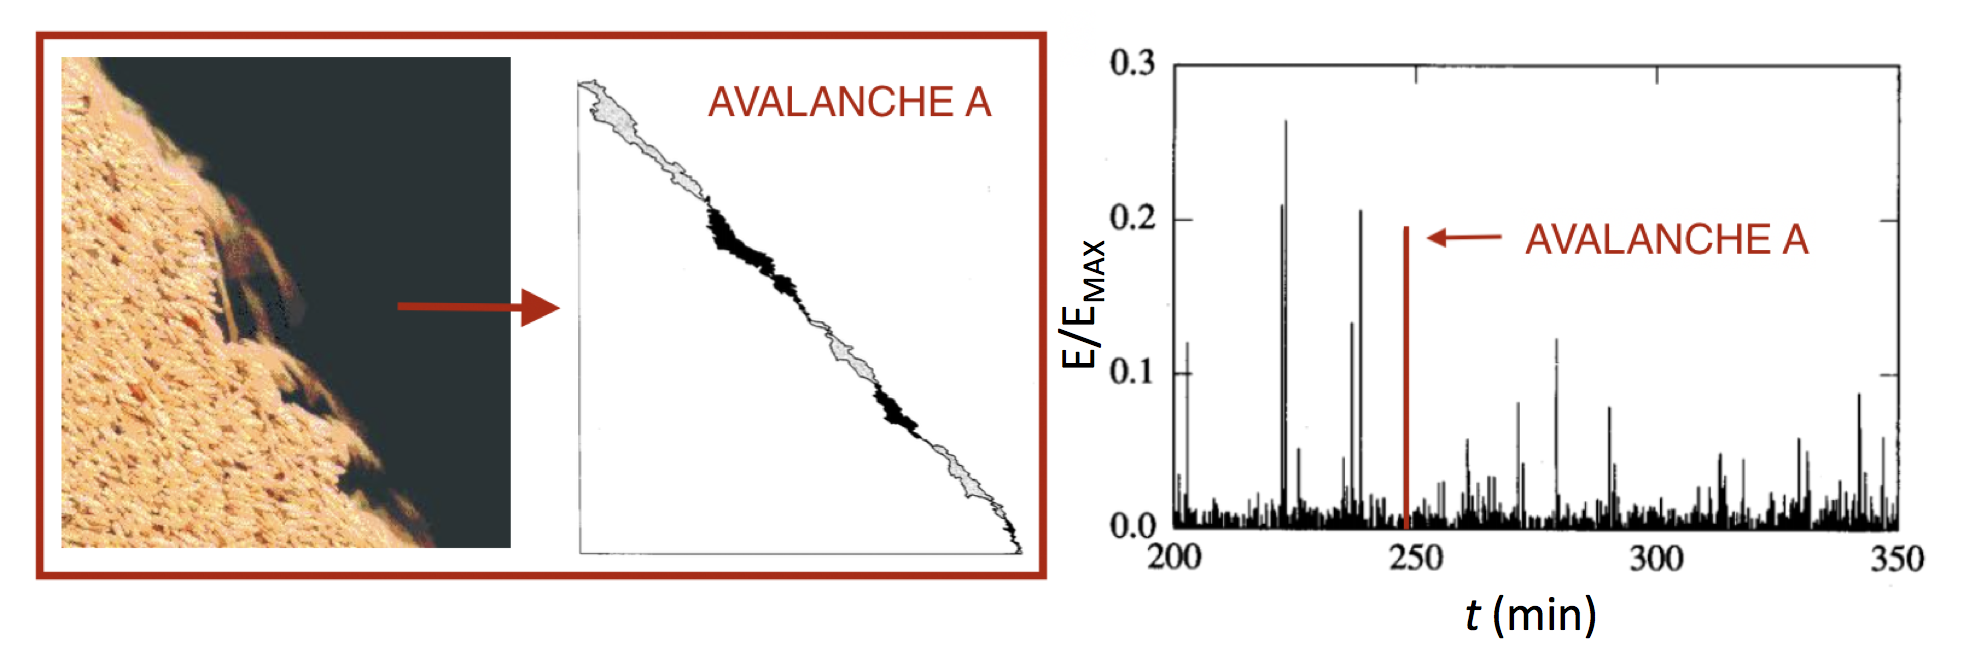
\includegraphics[width=0.95\textwidth]{Figures/Intro/riceFigs/riceEvent}
	\caption[Rice-pile Model]{
\textit{Rice pile model:} the photograph on the left shows an image of an avalanche occurring. The image before and after the avalanche are compared as shown by the middle image. This is used to calculate the size of the avalanche. The various avalanches that have occured in this run are plotted on the right. The images in this figure which have been modified were taken from \cite{riceExpt}. 
}
	\label{fig:perBak_cellular}
\end{figure*}

They repeated the experiment with two forms of rice grains, elongated rice grains and short rice grains. On taking data for several days, they were able to study the distribution of avalanches for both the types of rice grains. They found that the elongated rice grain pile exhibited SOC while the short ones did not - demonstrating that SOC is not universal \cite{riceExpt}. 
[To be completed]
%
%The distribution of energy dissipation events in this simple model is power-law distributed for a two-dimensional model. Similar models have been applied to explain the occurence of power-law event sizes in systems as diverse as earthquakes, front depinning and biological evolution.
%
%The original rice pile experiment measured the internal energy dissipation in a pile of rice confined between two glass plates. The energy of the pile was found by taking pictures of the pile from the side and calculating the potential energy from the distribution of mass in the pile. The experiment showed that for elongated grains of rice, the distribution of avalanche sizes were described by a power-law. However, for rounder grains the distribution was best described as a stretched exponential distribution with a characteristic size. It was speculated that the difference was due to differences in inertial effects in the two systems. However, the main conclusion was the self-organized criticality can be relevant to the description of granular systems, but it is not a universal behavior.
%
%The experiment was performed in several stages. During the first experimental period, pictures of the pile were taken with a video camera. However, it turned out that the spatial resolution and the stability of the video signal was not good enough to produce a reasonable scaling range for the measured energy. A second series of experiments were therefore performed with a \$100.000 CCD camera with a striking 2000x2000 spatial resolution with 12 bits of grayscale resolution was used. However, even with this camera, the system size was limited. In order to ascertain that very large piles did not behave significantly different, as have been claimed by several researchers, an experiment was performed on a 2.5m times 3m pile. The pile did not behave significantly different than the 80cm wide pile tested previously.


%One of the first empirical tests of Bak’s sand pile model took place in 1992, in the physics department of the University of Oslo. The physicists confined piles of rice between glass plates and added grains one at a time, capturing the resulting avalanche dynamics on camera. They found that the piles of elongated grains of rice behaved much like Bak’s simplified model.
%Most notably, the smaller avalanches were more frequent than the larger ones, following the expected power law distribution. That is, if there were 100 small avalanches involving only 10 grains during a given time frame, there would be 10 avalanches involving 100 grains in the same period, but only a single large avalanche involving 1,000 grains. (The same pattern had been observed in


\section{The Experiment}
[Will discuss the Wooster bead pile experiment ]

\section{Simulation}
\subsection{Previous Work}
[Ben Harris Code]
[Unity Simulation]
\subsection{Speed Boosts with GPUs}
[Examples of how GPU may help]
\subsection{Unified Particle Physics and Position Based Dynamics}
[What this is and why this would help us]


\section{Overview of Thesis}


\chapter{Theory}

\section{SOC and the Power Law}
\section{Physics of the Experimental System}
\subsubsection{Effect of Drop Height}
\subsubsection{Effect of Cohesion}
\subsection{Angle of Repose}
\subsection{Cohesion between Beads}

\section{How to take Advantage of GPUs}
\subsection{GPUs traditional role in Computers}
\subsection{Parallelising Code and Threading}

\section{Algorithms Used}
\subsection{Boundary Volume Hierarchy}
\subsection{Position-Based Dynamics}
\subsection{Unified-Particle Solving}

\chapter{Results}
\section{Comparing Simulation to Experiment}
Figure~\ref{fig:comparingData} contains plots of the data from the actual experiment on the left and the simulation on the right. There appears to be a similar trend present in the data sets, which is that there are periods of increasing mass and then a decrease in the mass (an avalanche). This is promising but we still need to acquire more data from the simulation before we can make statements about it.  Additionally, it is important to note that the initial parameters of both the experiment and the simulation that were used to obtain the data presented in the graphs are different. In the experiment, the drop height was set to be 2 cm. Additionally, the number of beads on the pile was about $1500$ beads. For the simulation, the drop height was 5 cm and there were $\sim60$K particles on the pile. 
\begin{figure*}[h]
	\centering
	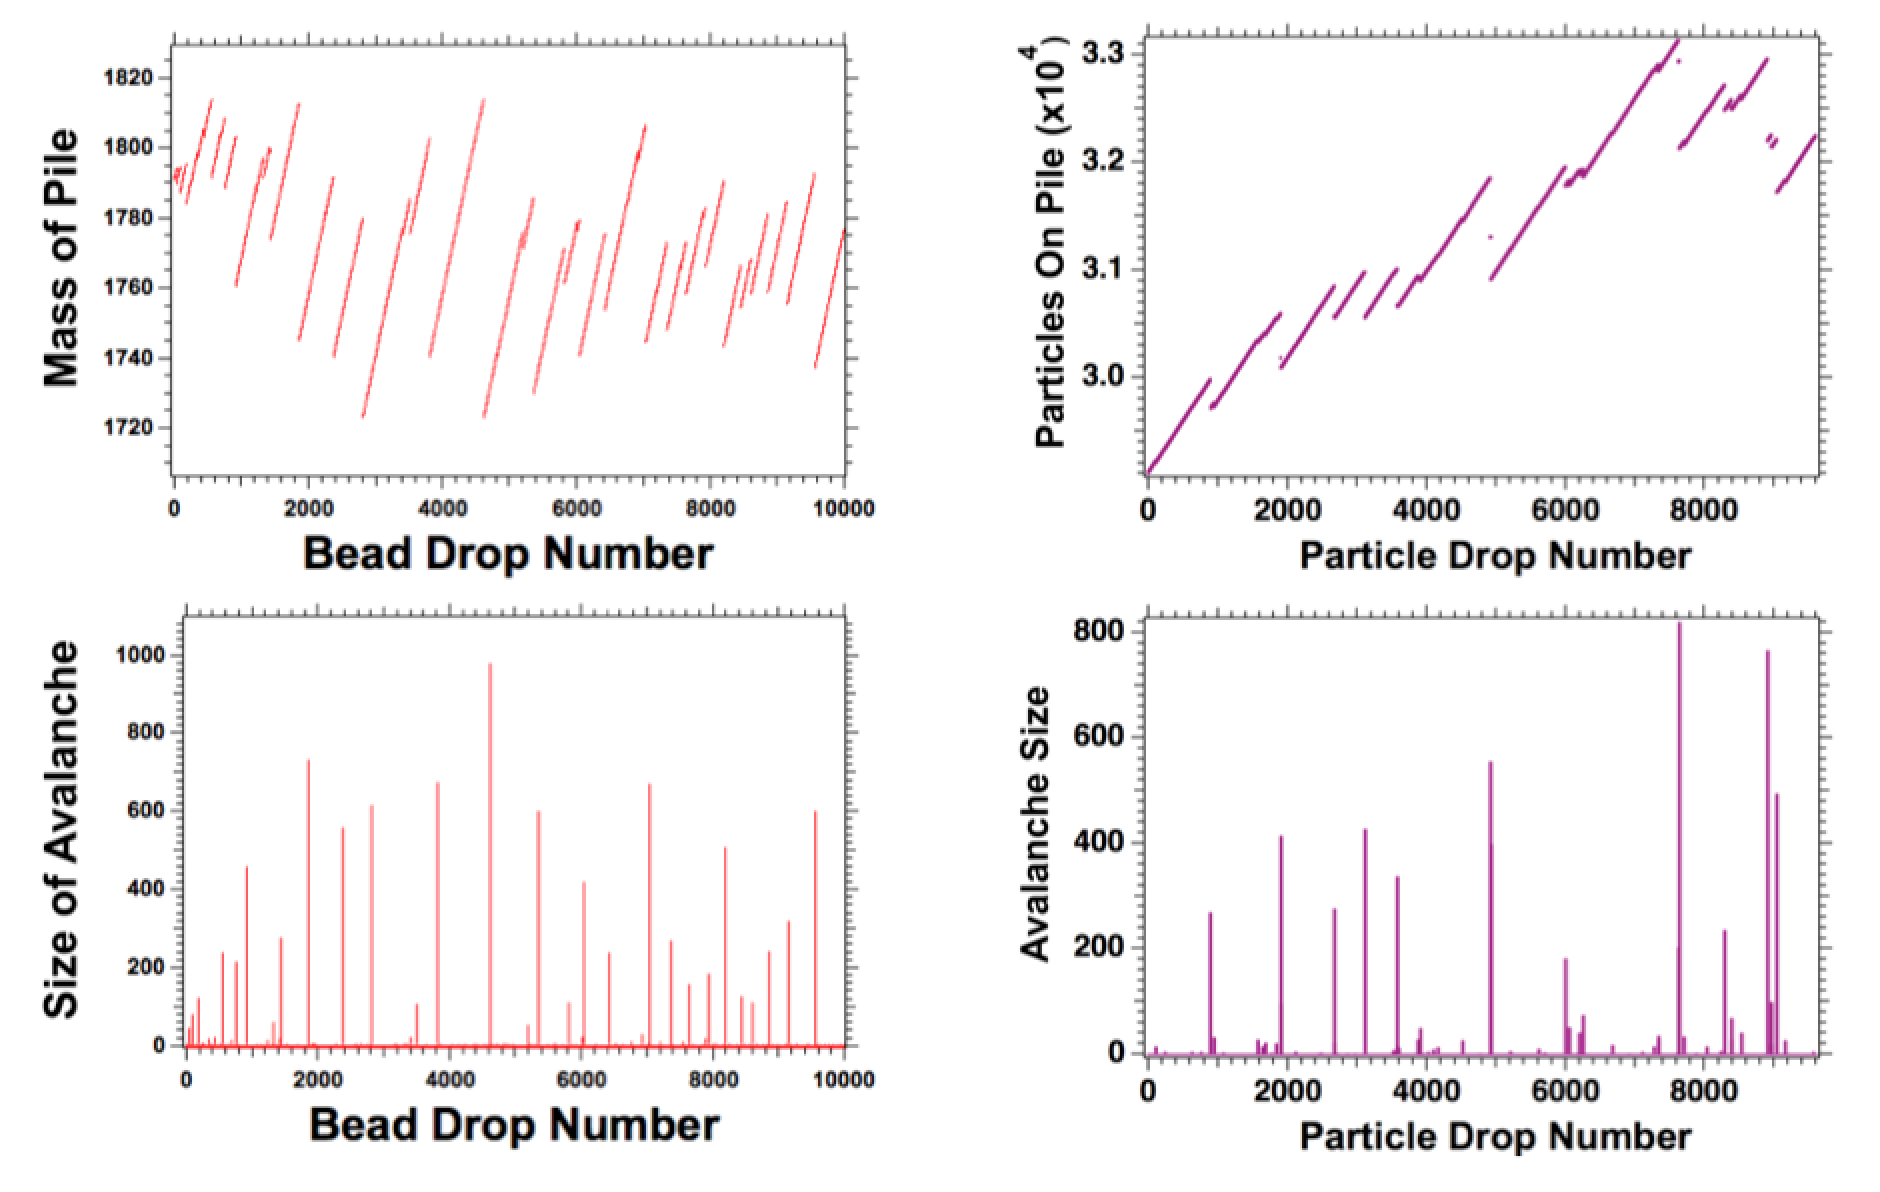
\includegraphics[width=0.95\textwidth]{Figures/Results/comparingData/origComparision}
	\caption[Comparing experiment and simuation data]{\textit{A comparison of data from the experiment and the simulation:} the plots on the right has been obtained from the experiment while the plots on the left have been obtained from the simulation. The plots on the top shows the mass/number of particles that constitutes the pile. The plots on the bottom shows the sizes of the avalanches that occur and the times at which the avalanches occur.}
	\label{fig:comparingData}
\end{figure*}

Figure~\ref{fig:energy} contains a plot of another data set acquired from the simulation. The plot on the bottom is that of the average kinetic energy of the pile. It is interesting to note that the average kinetic energy of the pile peaks when avalanches occur. This is something which we expect to occur as during the avalanche, a lot of beads will be moving. 
\begin{figure*}[h]
	\centering
	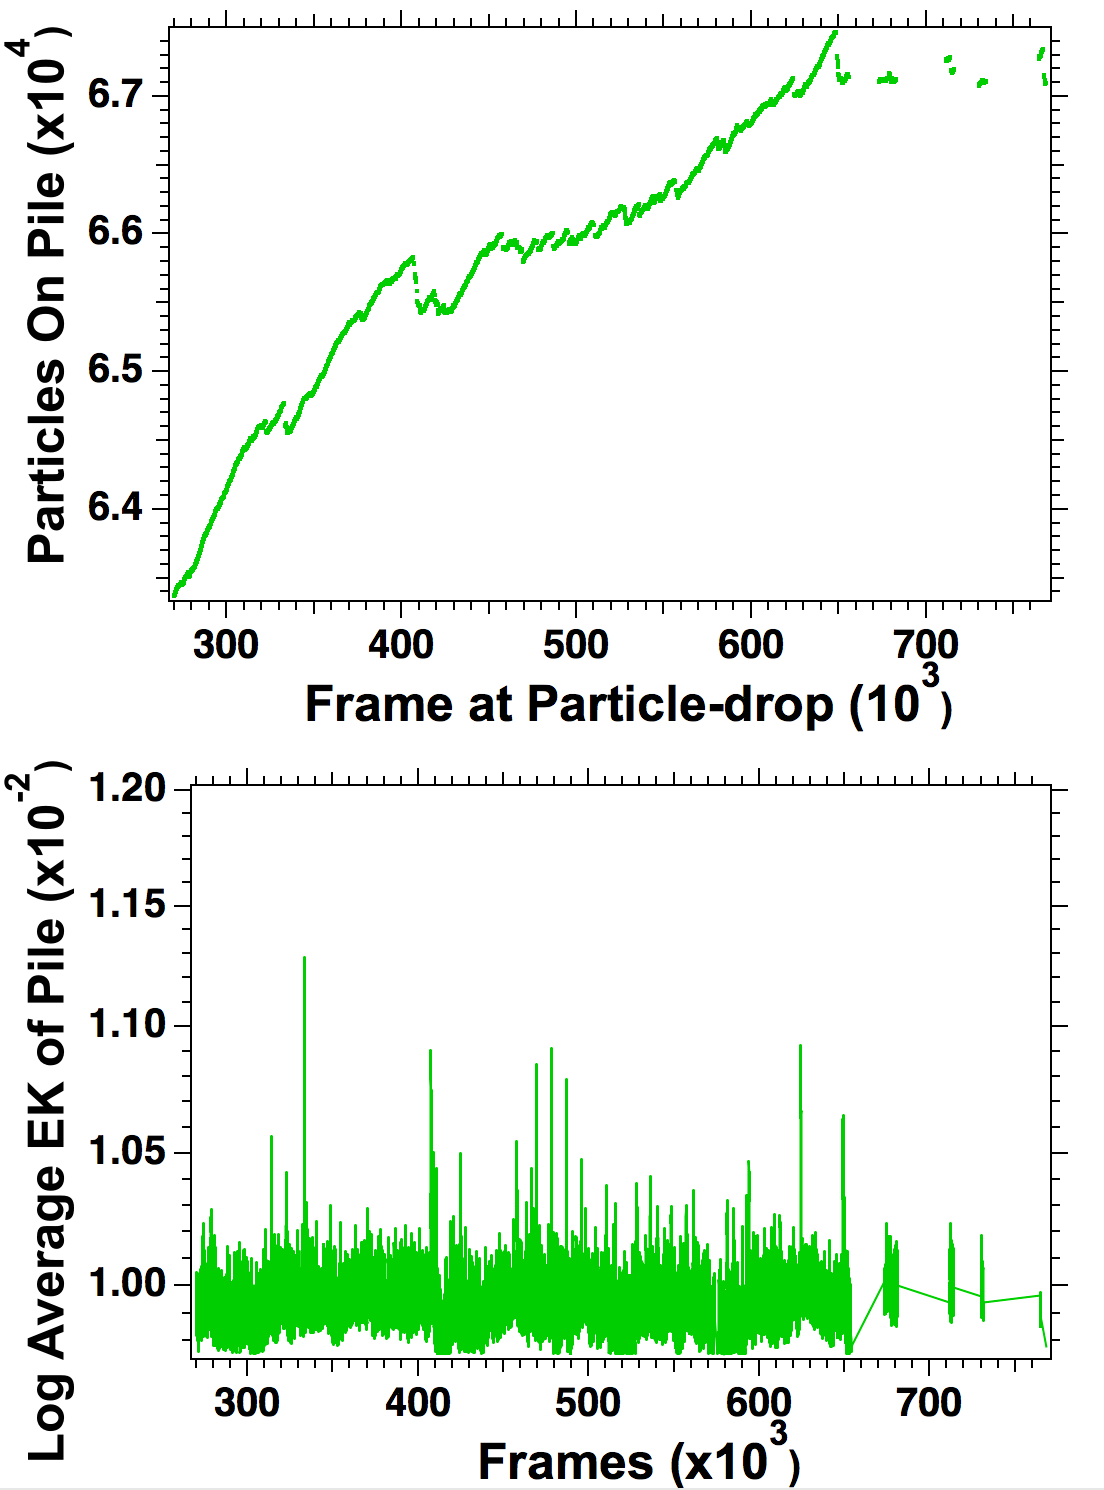
\includegraphics[width=0.95\textwidth]{Figures/Results/energy/e1}
	\caption[Average kinetic energy of simulated pile ]{\textit{Average kinetic energy of simulated pile:} the plot on the bottom shows the average kinetic energy of the pile. This can be used to determine when avalanches occur (average kinetic energy peaks when avalanches occur). This cannot be studied with the actual experiment. }
	\label{fig:energy}
\end{figure*}

%energy

\section{Testing the Simulation}
\subsection{Does it qualitatively appear realistic}
\subsection{Does it display a power law}
\subsection{Does it deviate from the power law with height/cohesion}

\section{Novel Results}



%%%%%%%%%%%%%%%%%%%%%%%%%%%%%%%%%%%%%%%%
%%%%%%%%%%%%%%%%%%%%%%%%%%%%%%%%%%%%%%%%
\chapter{Conclusions}\label{Conclusions}

\section{Stuff}


%%%%%%%%%%%%%%%%%%%%%%%%%%%%%%%%%%%%%%%%
%%%%%%%%%%%%%%%%%%%%%%%%%%%%%%%%%%%%%%%%
\appendix

\noappendicestocpagenum	 % suppress page number ...
\addappheadtotoc	% ... but add appendices header to table of contents 

\renewcommand{\theequation}{A-\arabic{equation}} % redefine the command that creates the equation number
\setcounter{equation}{0}  % reset counter 

\renewcommand{\thesection}{A-\arabic{section}} % redefine the command that creates the section number
\setcounter{section}{0}  % reset counter 

\renewcommand{\thetable}{A-\arabic{table}} % redefine the command that creates the table number
\setcounter{table}{0}  % reset counter 

%%%%%%%%%%%%%%%%%%%%%%%%%%%%%%%%%%%%%%%%
%%%%%%%%%%%%%%%%%%%%%%%%%%%%%%%%%%%%%%%%
\chapter{Extra Stuff}\label{Extra}

This is dummy text. This is dummy text. This is dummy text. This is dummy text. This is dummy text. This is dummy text. This is dummy text. This is dummy text. This is dummy text. This is dummy text. This is dummy text. This is dummy text. This is dummy text. This is dummy text. This is dummy text. This is dummy text. This is dummy text. This is dummy text. This is dummy text. This is dummy text. This is dummy text. This is dummy text. This is dummy text. This is dummy text. This is dummy text. This is dummy text. 

This is dummy text. This is dummy text. This is dummy text. This is dummy text. This is dummy text. This is dummy text. This is dummy text. This is dummy text. This is dummy text. This is dummy text. This is dummy text. This is dummy text. This is dummy text. This is dummy text. This is dummy text. This is dummy text. This is dummy text. This is dummy text. This is dummy text. This is dummy text. This is dummy text. This is dummy text. This is dummy text. This is dummy text. This is dummy text. This is dummy text. elegant text. This elegant text. This elegant text. This elegant text. This elegant text. 

%%%%%%%%%%%%%%%%%%%%%%%%%%%%%%%%%%%%%%%%
%%%%%% *-%%%%%%%%%%%%%%%%%%%%%%%%%%%%%%%%%
\chapter{Extra Stuffing}\label{Stuffing}
This is dummy text. This is dummy text. This is dummy text. This is dummy text. This is dummy text. This is dummy text. This is dummy text. This is dummy text. This is dummy text. This is dummy text. This is dummy text. This is dummy text. This is dummy text. This is dummy text. This is dummy text. This is dummy text. This is dummy text. This is dummy text. This is dummy text. This is dummy text. This is dummy text. This is dummy text. This is dummy text. This is dummy text. This is dummy text. This is dummy text. 

This is dummy text. This is dummy text. This is dummy text. This is dummy text. This is dummy text. This is dummy text. This is dummy text. This is dummy text. This is dummy text. This is dummy text. This is dummy text. This is dummy text. This is dummy text. This is dummy text. This is dummy text. This is dummy text. This is dummy text. This is dummy text. This is dummy text. This is dummy text. This is dummy text. This is dummy text. This is dummy text. This is dummy text. This is dummy text. This is dummy text. 

%%%%%%%%%%%%%%%%%%%%%%%%%%%%%%%%%%%%%%%%
%%%%%%%%%%%%%%%%%%%%%%%%%%%%%%%%%%%%%%%%
%%%%%%%%%%%%%%%%%%%%%%%%%%%%%%%%%%%%%%%%
\backmatter

\nocite{*}
\addcontentsline{toc}{chapter}{Bibliography}
\bibliography{thesis}
%\bibliographystyle{plain}			% listed alphabetically but ordered numerically, including titles
\bibliographystyle{unsrt}			% like plain but references appear in order of citation
%\bibliographystyle{alpha}		% like plain, except reference labels used
%\bibliographystyle{abbrv}		% like plain, but abbreviations uses for authors first names, etc.

\end{document}